%\documentclass[twocolumn,showpacs,preprintnumbers,amsmath,amssymb, floatfix]{revtex4}
\documentclass[aps,prb,preprint,preprintnumbers,amsmath,amssymb,floatfix,superscriptaddress]{revtex4}
%\documentclass[aps,prb,twocolumn,superscriptaddress,preprintnumbers,amsmath,amssymb,floatfix]{revtex4}

\usepackage{graphicx}
\usepackage{epstopdf}
\usepackage{ifthen}
\usepackage{dcolumn}
\usepackage{bm}
\usepackage{multirow}
\usepackage{booktabs}
\usepackage{amsbsy}
\usepackage{amsmath}
\usepackage{amssymb}
\usepackage{subfigure}
\usepackage{booktabs}

\graphicspath{
{/home/schuberm/Dropbox/git/plots.nogit/images}
}

%Definition of new commands
\newcommand{\f}[2]{\ensuremath{\frac{\displaystyle{#1}}{\displaystyle{#2}}}}
\newcommand{\lr}[1]{\langle{#1}\rangle}
\newcommand{\colv}[2] {\left(\begin{array}{c} #1 \\ #2 \end{array}\right)}
\renewcommand{\thefootnote}{\fnsymbol{footnote}}
\newcommand{\be} {\begin{eqnarray}}
\newcommand{\ee} {\end{eqnarray}}
%--------------------------------------------------------------------------
%EQ COMMANDS
%--------------------------------------------------------------------------
\newcommand{\two}{\mspace{-2.0mu}}
\newcommand{\four}{\mspace{-4.0mu}}
\newcommand{\plus}{\mspace{-4.5mu}+\mspace{-3.5mu}}
\newcommand{\minus}{\mspace{-4.5mu}-\mspace{-3.5mu}}
\newcommand{\pp}{'\mspace{-2.0mu}'}
\newcommand{\xlb}[4]{#1\ifthenelse{\equal{#2}{0}}{}{_{\alpha #2}}
\mspace{-2.0mu}\genfrac{(}{)}{0pt}{1}{\ifthenelse{\equal{#3}{0}}{0}{l #3}} 
{\ifthenelse{\equal{#4}{0}}{0}{b #4}}}

\newcommand{\xkv}[4]{#1\mspace{-5.0mu}\left(\mspace{-8.0mu}
\begin{smallmatrix}#2\four{}\four{}\mspace{-8.0mu}&\pmb{\kappa}#3\\&\nu 
#4\end{smallmatrix}\mspace{-5.0mu}\right)}

\newcommand{\evect}[6]{#1\mspace{-4.0mu}\left(\mspace{-8.0mu}
\begin{smallmatrix}#2\mspace{-8.0mu}&\pmb{\kappa} #3 &b #5\\&\nu #4 &
\alpha #6\end{smallmatrix}\mspace{-5.0mu}\right)}

\newcommand{\varmat}[8]{\mspace{-5.0mu}\left(\mspace{-8.0mu}
\begin{smallmatrix}\ifthenelse{\equal{#3}{0}}{\mspace{-8.0mu}&b_{#1}&b_{#2}
\\&\alpha_{#1}&\alpha_{#2}} {\ifthenelse{\equal{#7}{0}}{#1\mspace{-8.0mu}&
\pmb{\kappa}#2#3\mspace{-8.0mu}&\pmb{\kappa}#4#5\mspace{-8.0mu}&\pmb{\kappa}
#6\\&\nu#2&\nu#4&\nu#6} {#1\mspace{-8.0mu}&\pmb{\kappa}#2#3\mspace{-8.0mu}&
\pmb{\kappa}#4#5\mspace{-8.0mu}&\pmb{\kappa}#6#7\mspace{-8.0mu}&\pmb{\kappa}
#8\\&\nu#2&\nu#4&\nu#6&\nu#8}}\end{smallmatrix}\mspace{-5.0mu}\right)}

\newcommand{\EXP}[1]{\exp\mspace{-5.0mu}\left[#1\right]\mspace{-3.0mu}}

\newcommand{\tpp}[2]{\left(\mspace{-2.0mu}\xkv{\omega}{}{}{}#1\xkv{\omega}
{}{'}{'}#2\xkv{\omega}{}{\pp}{\pp}\mspace{-2.0mu}\right)}

\newcommand{\SUM}[2]{\ifthenelse{\equal{#1}{0}}{\sum_{
\alpha_{#2},b_{#2},l_{#2}}^{3,n,N}} {\ifthenelse{\equal{#1}{1}}{\sum_{
\alpha_{#2},b_{#2}}^{3,n}}{\sum_{\pmb{\kappa}#2,\nu#2}^{N,3n}}}}

\newcommand{\SUMprime}[2]{\ifthenelse{\equal{#1}{0}}
{\sum_{\alpha_{#2},b_{#2},l_{#2}}^{3,n,N}} 
{\ifthenelse{\equal{#1}{1}}{\sum_{\alpha_{#2},b_{#2}}^{3,n}}
{\sum_{\pmb{\kappa}^{'}#2,\nu#2}^{N,3n}}}}

\newcommand{\SUMalpha}[2]{\ifthenelse{\equal{#1}{0}}
{\sum_{\alpha_{#2}}^{3}} {\ifthenelse{\equal{#1}{1}}
{\sum_{\alpha_{#2},b_{#2}}^{3,n}}{\sum_{\pmb{\kappa}#2,\nu#2}^{N,3n}}}}

\newcommand{\SUMalphap}[2]{\ifthenelse{\equal{#1}{0}}
{\sum_{\alpha'_{#2}}^{3}} {\ifthenelse{\equal{#1}{1}}
{\sum_{\alpha'_{#2},b'_{#2}}^{3,n}}{\sum_{\pmb{\kappa}#2,\nu#2}^{N,3n}}}}

\newcommand{\SUMb}[2]{\ifthenelse{\equal{#1}{0}}{\sum_{b_{#2}}^{n}}
 {\ifthenelse{\equal{#1}{1}}{\sum_{\alpha_{#2},b_{#2}}^{3,n}}
{\sum_{\pmb{\kappa}#2,\nu#2}^{N,3n}}}}

\newcommand{\SUMbp}[2]{\ifthenelse{\equal{#1}{0}}{\sum_{b'_{#2}}^{n}}
 {\ifthenelse{\equal{#1}{1}}{\sum_{\alpha'_{#2},b'_{#2}}^{3,n}}
{\sum_{\pmb{\kappa}#2,\nu#2}^{N,3n}}}}

\newcommand{\SUMl}[2]{\ifthenelse{\equal{#1}{0}}{\sum_{l_{#2}}^{N}}
 {\ifthenelse{\equal{#1}{1}}{\sum_{\alpha_{#2},b_{#2}}^{3,n}}
{\sum_{\pmb{\kappa}#2,\nu#2}^{N,3n}}}}

\newcommand{\SUMlp}[2]{\ifthenelse{\equal{#1}{0}}{\sum_{l'_{#2}}^{N}}
 {\ifthenelse{\equal{#1}{1}}{\sum_{\alpha'_{#2},b'_{#2}}^{3,n}}
{\sum_{\pmb{\kappa}#2,\nu#2}^{N,3n}}}}

\newcommand{\abcdt}[5]{\mspace{-4.0mu}\left(\mspace{-8.0mu}
\begin{smallmatrix}&\ifthenelse{\equal{#1}{}}{a}{#1}&\ifthenelse
{\equal{#3}{}}{c}{#3}\\&\ifthenelse{\equal{#2}{}}{b}{#2}&\ifthenelse
{\equal{#4}{}}{d}{#4}\end{smallmatrix}\mspace{-2.0mu};\ifthenelse
{\equal{#5}{}}{t}{#5}\right)}

\newcommand{\abcd}[4]{\mspace{-4.0mu}\left(\mspace{-8.0mu}
\begin{smallmatrix}&\ifthenelse{\equal{#1}{}}{a}{#1}&\ifthenelse
{\equal{#3}{}}{c}{#3}\\&\ifthenelse{\equal{#2}{}}{b}{#2}&\ifthenelse
{\equal{#4}{}}{d}{#4}\end{smallmatrix}\mspace{-3.0mu}\right)}

\newcommand{\abt}[3]{\mspace{-4.0mu}\left(\mspace{-8.0mu}\begin
{smallmatrix}&\ifthenelse{\equal{#1}{}}{a}{#1} \\&\ifthenelse{
\equal{#2}{}}{b}{#2}\end{smallmatrix}\mspace{-2.0mu};
\ifthenelse{\equal{#3}{}}{t}{#3}\right)}

\newcommand{\ab}[2]{\mspace{-4.0mu}\left(\mspace{-8.0mu}
\begin{smallmatrix}&\ifthenelse{\equal{#1}{}}{a}{#1} \\&\ifthenelse
{\equal{#2}{}}{b}{#2}\end{smallmatrix}\mspace{-3.0mu}\right)}

\newcommand{\kvbat}{\mspace{-4.0mu}\left(\mspace{-8.0mu}
\begin{smallmatrix} &\pmb{\kappa} &b \\ &\nu &\alpha\end{smallmatrix}
\mspace{-2.0mu};t\right)}

\newcommand{\kvbatp}{\mspace{-4.0mu}\left(\mspace{-8.0mu}
\begin{smallmatrix} &\pmb{\kappa} &b' \\ &\nu &\alpha'\end{smallmatrix}
\mspace{-2.0mu};t\right)}

\newcommand{\kvbaw}{\mspace{-4.0mu}\left(\mspace{-8.0mu}
\begin{smallmatrix} &\pmb{\kappa} &b \\ &\nu &\alpha\end{smallmatrix}
\mspace{-2.0mu};\omega\right)}

\newcommand{\kvbawp}{\mspace{-4.0mu}\left(\mspace{-8.0mu}
\begin{smallmatrix} &\pmb{\kappa} &b' \\ &\nu &\alpha'\end{smallmatrix}
\mspace{-2.0mu};\omega\right)}

\newcommand{\kvba}{\mspace{-4.0mu}\left(\mspace{-8.0mu}
\begin{smallmatrix} &\pmb{\kappa} &b \\ &\nu &\alpha\end{smallmatrix}
\mspace{-3.0mu}\right)}

\newcommand{\kvbap}{\mspace{-4.0mu}\left(\mspace{-8.0mu}
\begin{smallmatrix} &\pmb{\kappa}' &b \\ &\nu' &\alpha\end{smallmatrix}
\mspace{-3.0mu}\right)}

\newcommand{\kpvba}{\mspace{-4.0mu}\left(\mspace{-8.0mu}
\begin{smallmatrix} &\pmb{\kappa}^{'} &b \\ &\nu &\alpha\end{smallmatrix}
\mspace{-3.0mu}\right)}

\newcommand{\kva}{\mspace{-4.0mu}\left(\mspace{-8.0mu}
\begin{smallmatrix} &\pmb{\kappa} \\ &\nu &\alpha\end{smallmatrix}
\mspace{-3.0mu}\right)}

\newcommand{\kvap}{\mspace{-4.0mu}\left(\mspace{-8.0mu}
\begin{smallmatrix} &\pmb{\kappa} \\ &\nu &\alpha'\end{smallmatrix}
\mspace{-3.0mu}\right)}

\newcommand{\kvb}{\mspace{-4.0mu}\left(\mspace{-8.0mu}
\begin{smallmatrix} &\pmb{\kappa} &b \\ &\nu \end{smallmatrix}
\mspace{-3.0mu}\right)}

\newcommand{\kvbp}{\mspace{-4.0mu}\left(\mspace{-8.0mu}
\begin{smallmatrix} &\pmb{\kappa} &b' \\ &\nu \end{smallmatrix}
\mspace{-3.0mu}\right)}

\newcommand{\kvt}{\mspace{-4.0mu}\left(\mspace{-8.0mu}
\begin{smallmatrix}&\pmb{\kappa} \\&\nu\end{smallmatrix}
\mspace{-2.0mu};t\right)}

\newcommand{\kvzero}{\mspace{-4.0mu}\left(\mspace{-8.0mu}
\begin{smallmatrix}&\pmb{\kappa} \\&\nu\end{smallmatrix}
\mspace{-2.0mu};0\right)}

\newcommand{\kpvt}{\mspace{-4.0mu}\left(\mspace{-8.0mu}
\begin{smallmatrix}&\pmb{\kappa}^{'} \\&\nu\end{smallmatrix}
\mspace{-2.0mu};t\right)}

\newcommand{\kvw}{\mspace{-4.0mu}\left(\mspace{-8.0mu}
\begin{smallmatrix}&\pmb{\kappa} \\&\nu\end{smallmatrix}
\mspace{-2.0mu};\omega\right)}

\newcommand{\kv}{\mspace{-4.0mu}\left(\mspace{-8.0mu}
\begin{smallmatrix}&\pmb{\kappa} \\&\nu\end{smallmatrix}
\mspace{-3.0mu}\right)}

\newcommand{\kvp}{\mspace{-4.0mu}\left(\mspace{-8.0mu}
\begin{smallmatrix}&\pmb{\kappa'} \\&\nu'\end{smallmatrix}
\mspace{-3.0mu}\right)}

\newcommand{\kw}{\mspace{-4.0mu}\left(\mspace{-8.0mu}
\begin{smallmatrix}&\pmb{\kappa} \\&\omega\end{smallmatrix}
\mspace{-3.0mu}\right)}

\newcommand{\kpvp}{\mspace{-4.0mu}\left(\mspace{-8.0mu}
\begin{smallmatrix}&\pmb{\kappa'} \\&\nu'\end{smallmatrix}
\mspace{-3.0mu}\right)}

\newcommand{\lbt}{\mspace{-4.0mu}\left(\mspace{-8.0mu}
\begin{smallmatrix}&l \\&b\end{smallmatrix}\mspace{-2.0mu};t\right)}

\newcommand{\lbtp}{\mspace{-4.0mu}\left(\mspace{-8.0mu}
\begin{smallmatrix}&l' \\&b'\end{smallmatrix}\mspace{-2.0mu};t\right)}

\newcommand{\lt}{\mspace{-4.0mu}\left(\mspace{-8.0mu}
\begin{smallmatrix}&l\end{smallmatrix}\mspace{-2.0mu};t\right)}

\newcommand{\ltp}{\mspace{-4.0mu}\left(\mspace{-8.0mu}
\begin{smallmatrix}&l'\end{smallmatrix}\mspace{-2.0mu};t\right)}

\newcommand{\lb}{\mspace{-4.0mu}\left(\mspace{-8.0mu}
\begin{smallmatrix}&l \\&b\end{smallmatrix}\mspace{-3.0mu}\right)}

\newcommand{\lbp}{\mspace{-4.0mu}\left(\mspace{-8.0mu}
\begin{smallmatrix}&l' \\&b'\end{smallmatrix}\mspace{-3.0mu}\right)}
%--------------------------------------------------------------------------
%END COMMANDS
%--------------------------------------------------------------------------
%--------------------------------------------------------------------------
\begin{document}

\title{Mean Free Paths of Superlattice Phonons}
\author{Samuel C. Huberman}
\affiliation{Department of Mechanical \& Industrial Engineering, University of Toronto, 
Toronto, Ontario M5S 3G8, Canada}
\author{Jason M. Larkin}
\affiliation{Department of Mechanical Engineering\\Carnegie Mellon University\\Pittsburgh, PA 15213}
\author{Alan J. H. McGaughey}
%\email{mcgaughey@cmu.edu}
\affiliation{Department of Mechanical Engineering\\Carnegie Mellon University\\Pittsburgh, PA 15213}
\author{Cristina H. Amon}
\affiliation{Department of Mechanical \& Industrial Engineering, University of Toronto, 
Toronto, Ontario M5S 3G8, Canada}
\affiliation{Department of Mechanical Engineering\\Carnegie Mellon University\\Pittsburgh, PA 15213}

\date{\today}% It is always \today, today,
             %  but any date may be explicitly specified
\vspace{14mm}
  
\begin{abstract}

We use normal mode decomposition to obtain phonon properties from quasi-harmonic lattice dynamics calculations and classical molecular dynamics simulations in unstrained Lennard-Jones argon superlattices. The relaxation-time approximation of the Boltzmann transport equation is used to predict cross-plane and in-plane thermal conductivity for a range of superlattice period lengths. Debye scaling ($\omega^{-2}$) of phonon lifetimes is found a low frequencies and Rayleigh scaling ($\omega^{-4}$) for intermediate frequencies in superlattices with interfacial mixing. We find that interspecies mixing reduces a phonon's mean free path and for short-period superlattices, lifetimes below the Ioffe-Regel limit are observed.

\end{abstract}
\maketitle
%%%%
\section{Introduction}
Equilibrium \cite {PhysRevB.85.195302} and non-equilibrium \cite {PhysRevB.79.214307,PhysRevB.79.075316,PhysRevB.72.174302} studies have been performed on a variety of superlattices. Although these techniques make predictions about the trends of thermal conductivity, a mode by mode analysis is required to understand the effects of the secondary periodicity upon phonon properties. Prior models relied upon approximations of the specularity and diffusivity of the interfaces \cite {PhysRevB.57.14958} and lacked the computational power \cite {PhysRevB.70.081310}. Recent work \cite{Luckyanova16112012,doi:10.1021/nl202186y} used Density Functional Perturbation Theory. Unlike these works, where the phonon properties for short period superlattices is used for larger period superlattices for computational reasons \cite{Luckyanova16112012, doi:10.1021/nl202186y} or interfacial mixing is neglected \cite{doi:10.1021/nl202186y}, we demonstrate the ability of normal mode decomposition (NMD) to predict the phonon properties in unstrained superlattices with perfect and mixed interfaces without making such approximations about the dispersion.
%%%
\section{Modeling Framework}
%%%
Like previous superlattice studies \cite{Luckyanova16112012,doi:10.1021/nl202186y}, the phonon Boltzmann Transport Equation (BTE) under the single mode relaxation time approximation \cite{ziman_electrons_2001}, is used to predict the thermal conductivity in the $i$th direction
%%%
\begin{equation}\label{EQ:M:conductivity}
\begin{split}
k_{vib,\mathbf{i}}=&\sum_{\pmb{\kappa}} \sum_\nu c_{ph}\kv
\pmb{v}^{2}_{g,\mathbf{i}}\kv \tau\kv.
\end{split}
\end{equation}
%%%
To obtain the required inputs for the BTE, the phonon lifetime $\tau\kv$ and phonon group velocity, $\pmb{v}^{2}_{g,\mathbf{i}}\kv$, we follow the NMD procedure outlined by McGaughey\cite{PhysRevB.71.184305}, Turney \cite {PhysRevB.81.081411} and Larkin \cite{jason_inpress}. The basis of this mode by mode phonon analysis relies upon using the fundamental repeated unit of material, which for the superlattice, consisted of N conventional face centered cubic unit cells of $m_a$ and N unit cells of $m_b$ along the cross-plane direction, thus a $2\times2$ ($N\times N$) superlattices refers to a superlattice period of 2 (N) monolayers of $m_A$ and 2 (N) monolayers of $m_B$. Size effects were accounted for by performing a convergence study. It was found predictions in both cross-plane and in-plane thermal conductivities varied by less than 10\% for systems with more than $N_x=8$ superlattice UCs along the cross-plane and $N_y=N_z=6$ UCs along the in-plane ($N_x=10$ for $2\times2$ to resolve the lifetime scalings). No lattice strain was permitted as the effects have been studied elsewhere \cite{PhysRevB.72.174302}. 
%%%

\begin{figure*}[ht!]
\begin{center}
\scalebox{0.5}{ \includegraphics{/home/schuberm/Dropbox/git/plots.nogit/images/4p_ai.eps}}
\renewcommand{\figure}{Fig.}
\caption{Atomic representation of a $4\times4$ superlattice for perfect (top) and 80/20 (bottom) cases.}
\label{fig:dispersion}
\end{center}
\end{figure*}
%%%

Following the approach put forward by Landry \cite{PhysRevB.79.075316}, interspecies interfacial mixing was controlled by selecting the individual adjacent monolayers to an interface in the MD computational cell and flipping the masses of randomly selected atoms until the desired concentrations were reached. For example, a mixing of 80/20 refers an original/foreign blend in an adjacent monolayer. NMD calculations were conducted for a range of period lengths; $2\times2$, $4\times4$, $8\times8$ and $14\times14$ for Lennard-Jones argon superlattices with a mass ratio ($m_a/m_b$) of 3 at a temperature of 20 Kelvin. MD was conducted using the LAMMPS package \cite{LAMMPS}. The LJ potential was set to be the same for all possible pairwise interactions with $\epsilon= 1.67E-21$ J and $\sigma= 3.4E-10$ m. The remainder of this work uses dimensionless units unless otherwise noted ($E*=E/\epsilon$, $T*=Tk_B/\epsilon$, $\omega*=\omega\sqrt{\sigma^2m_a/\epsilon}$, $k*=km^{0.5}\sigma^2/(\epsilon^{0.5}k_B)$). The time step for molecular dynamics was set to 4.285 fs. The specific heat is set to be $k_B/V$ per mode, where V is the system volume of the molecular dynamics computational domain, because the systems considered here are classical and obey Maxwell-Boltzmann statistics. As temperature increases, anharmonicity of the potential energy decreases the specific heat from $\frac{k_B}{V}$. However, the effect is small for these superlattices at 20 K \cite{Jason}. The unit cells depicted in Fig. are used as inputs into harmonic lattice dynamics calculations, conducted using GULP \cite{GULP}. Group velocities were calculated using finite differencing about a given frequency. The allowed wavevectors, $\pmb{\kappa}$, are selected in accordance with the number of repetitions of the unit cell used in the classical molecular dynamics simulations
%%%
\begin{equation}\label{EQ:NMD:allowdkpt}
\pmb{\kappa} = \sum_{\alpha} \pmb{b}_{\alpha} \frac{n_{\alpha}}{N_{\alpha}},
\end{equation}
%%%
where $\pmb{b}_\alpha$ are the cubically orthogonal reciprocal lattice vectors and $ \frac{N_\alpha}{2} < n_\alpha \le \frac {N_\alpha}{2}$, where n are integers and N are now constant even integers. The wavevectors are taken to be in the first Brillouin zone. The eigenvectors, obtained from the lattice dynamics calculations, are used to construct a basis upon which the velocities are projected to obtain the time series of the time derivative of the normal mode coordinate 
%%%
\begin{equation}\label{EQ:NMD:qdot}
\begin{split}
\dot{q}\kvt{}{}{}=&\SUM{0}{}\sqrt{\frac{m_b}{N}}\dot{u}_{\alpha}\lbt e^*\kvba\EXP{i\pmb{\kappa}\cdot\mathbf{r}_0\ab{l}{0}},
\end{split}
\end{equation}
%%%
where $\dot{u}_{\alpha}\lbt$ is the component of velocity of atom $b$ in the $l$ th unit cell in the $\alpha$ direction and $e^*\kvba$ denotes the complex conjugate of the $\alpha$ component for atom $b$ of the eigenvector for mode $\kv$. By taking the Fourier transform of the autocorrelation of the time derivative of the normal mode coordinate, the power spectrum is resolved \cite{dove_introduction_1993-3}
%%%
\begin{equation}\label{EQ:NMD:SED}
\begin{split}
T\kvw=&\lim_{\tau_0\rightarrow\infty}\frac{1}{2\tau_0}\left|\frac{1}{\sqrt{2\pi}}\int_{0}^{\tau_0}\dot{q}\kvt\exp(-i\omega t)dt\right|^2.
\end{split}
\end{equation}
%%% 
The Fourier transform sampling window was set to $2^{16}$ time steps to capture modes with frequencies greater than 1 and a larger window of $2^{22}$ time steps was used for modes with frequencies less than 1. The lag between velocities samples was $2^5$ was found to be sufficient to capture the dynamics of highest frequency phonon modes. Five independent molecular dynamics simulations with different initial velocity seeds were run and the power spectrum was averaged over all seeds and Fourier transform sampling windows. Further averaging was conducted by imposing the symmetry of the irreducible Brillouin zone. In accordance with anharmonic theory, the power spectrum can be approximated to be a Lorentzian of the form for cases where $\Gamma\kv \ll \omega_0\kv$ \cite{maradudin_scattering_1962}
%%%
\begin{equation}\label{EQ:NMD:LOR}
\begin{split}
T\kvw\approx&C_0\kv\frac{\Gamma\kv/\pi}{[\omega_0\kv-\omega]^2+\Gamma^2\kv},
\end{split}
\end{equation}
%%%
and thus fitting Equation~\ref{EQ:NMD:LOR} to Equation~\ref{EQ:NMD:SED} yields the phonon lifetime
%%%
\begin{equation}\label{EQ:lifetime}
\begin{split}
\tau\kv=&\frac{1}{2\Gamma\kv}
\end{split}
\end{equation}
%%%
This spectral width corresponds to all possibles mechanisms of phonon interaction since no \textit{a priori} assumptions about such interactions were involved in its determination (and the effect of the secondary periodicity is captured by using the modified phonon dispersion). Thus all phonon-phonon scattering probabilities are enveloped into this single quantity. Fitting was done by only considering points within 3 orders of magnitude of the maximum value of the power spectrum. The initial guess for the linewidth ($\Gamma\kv$) of the Lorentzian was set to 0.01.
The phonon-phonon mean free path, in the phonon-as-a-particle interpretation, is typically defined as the distance travelled between particle collisions \cite{ziman_electrons_2001}. Coherence length is the distance a plane wave travels until the phase becomes uncorrelated and thus only applies in the wave picture of phonon transport. Phase is assumed to be randomized through inelastic phonon-phonon, but not elastic boundary or impurity scattering \cite{chen2005nanoscale}. However, other definitions argue that roughness and disorder, in general, destroy coherent effects \cite{PhysRevB.67.195311,dames:682}. Adopting a unit cell that spans one period to generate the modified dispersion relation allows one to ignore the difference between the MFP and coherence length
%%%
\begin{equation}\label{EQ:M:phonon_mfp}
\begin{split}
\Lambda\kv &= |\pmb{v}_{g}\kv {}| \tau\kv.
\end{split}
\end{equation}
%%%
To validate the phonon properties, anharmonic lattice dynamics \cite{PhysRevB.79.064301} (ALD) was performed on the unmixed systems with the equivalent resolution of the Brouillin zone. ALD perturbs the harmonic solutions from HLD to obtain phonon lifetimes. ALD cannot determine the effects of mixing because of the analysis is based in reciprocal space and as such imposes the same geometric mixing to all unit cells. Other superlattice studies \cite{Luckyanova16112012} have adopted the Tamura isotope scattering theory \cite{tamura_isotope_1983} to modify the ALD predicted lifetimes
%%%
\begin{equation}\label{EQ:tau_eff}
\begin{split}
\frac{1}{\tau_{eff}\kv} = \frac{1}{\tau_{d}\kv}+\frac{1}{\tau_{ald}\kv} ,
\end{split}
\end{equation}
%%%
where
%%%
\begin{equation}\label{EQ:tau_d}
\begin{split}
\frac{1}{\tau_{d}\kv} = \frac{\pi}{2N_{uc}}\omega^2\kv 
\sum_{\pmb{\kappa'}\nu'} \delta( \omega\kv - \omega\kvp )\sum_{b} g_2(b) 
|e^*\kvbap \cdot e\kvba |^2 ,
\end{split}
\end{equation}
%%%
and the term $g_2(b)$ is a coupling term which defines the strength of the mass disordering
%%%
\begin{equation}\label{EQ:g(b)}
\begin{split}
g_2(b) = \sum_\mu c^{\mu}(b)(1-m^{\mu}(b)/\bar{m}(b))^2, 
\end{split}
\end{equation}
%%%
$N_{uc}$ is the number of unit cells, and $c^\mu$ is the concentration of the mixing, $m^\mu(b)$ is the mass of the $\mu$-th species and $\bar{m}^{\mu}$ is the average mass. There is one atom type in the unit cell with $\mu=a,b$, so that the alloying atom labeled by $m^b_{1-c}$ can be considered to be an ``isotope'' of atom labeled $m^a_{c}$. 
%This convention is appropriate because of the perturbative approach used to derive Eq. ~\ref{TB:tau_d}, while we consider large disorder up to $c=0.5$.\cite{tamura_isotope_1983} 

Green-Kubo (GK) simulations, previously validated against the non-equilibrium direct method \cite {PhysRevB.79.075316}, were performed on the the same molecular domain, for consistency, that was used in the NMD approach for both mixed and non mixed systems. In order to minimize the error in the GK predictions, the relative error function of the heat current autocorrelation function (HCACF) was used to determine the point at which the cumulative integral of the HCACF converges \cite{Chen20102392}.

\section{Results}
The unit cells described in the previous section generate dispersions similar to what can be seen in Figure~\ref{fig:dispersion}, increasing the number of branches as the number of atoms in the unit cell increases. Mini or stop gaps emerge at the Brouillin zone edges as a consequence of the folding of the branches \cite{PhysRevB.38.1427} \cite{PhysRevB.60.2627}. The density of states shares the $\omega^2$ scaling at low frequencies as found with bulk LJ and Stilinger-Weber silicon systems \cite{}. 
%%%
\renewcommand{\topfraction}{0.7}
\begin{figure*}[ht!]
\begin{center}
\scalebox{1}{ \includegraphics{/home/schuberm/Dropbox/git/plots.nogit/images/4p_dispersion.eps}}
\renewcommand{\figure}{Fig.}
\caption{Dispersion of a 4x4 superlattice for modes normal to the interfaces. Red squares represent select modes for $\pmb{\kappa}$=[1,0,0].}
\label{fig:dispersion}
\end{center}
\end{figure*}
%%%
Selected sample power spectrums are shown in Figure~\ref{fig:sed}. Note that while the peaks appear to be Lorentzian centered about single frequency, there are minor signatures at other frequencies. These signatures are attributed to the approximation that the normal mode of the harmonic system is equivalent to the normal mode of the anharmonic system. In the interfacial mixing cases, the intensity of the signatures becomes amplified, an indication of the shared implications of disorder (random masses with linear springs) and anharmonicity (ordered masses with non-linear springs) \cite{RevModPhys.53.175} upon phonon propagation, as experienced by electrons \cite{mott1961theory}. The degenerate modes 20 and 21 experience large disruption. This may be the result of the large number of modes with similar frequencies, observed in the density of states shown in Figure~\ref{fig:dispersion} at around $\omega=15$, available for these modes to interact within a differential of frequency, as described in Allen-Feldmann theory \cite{allen_thermal_1993,feldman_thermal_1993-1}.
%%%
\begin{figure}[!h]
\begin{center}
\scalebox{1}{ 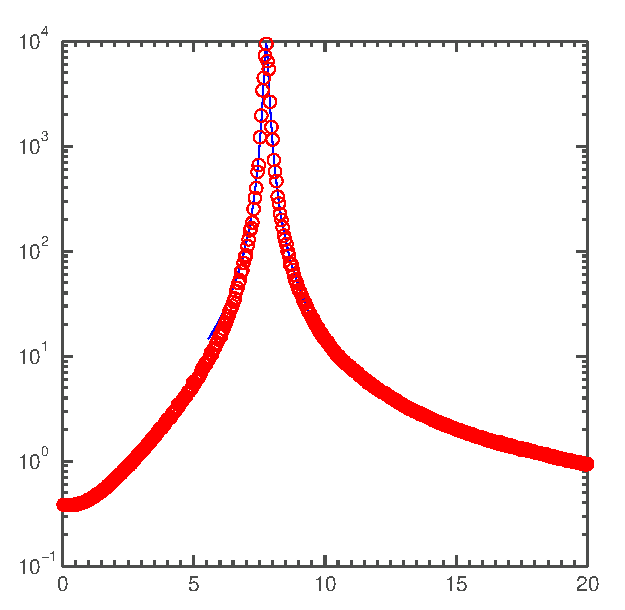
\includegraphics{/home/schuberm/Dropbox/git/plots.nogit/images/sed.eps}}
\renewcommand{\figure}{Fig.}
\caption{(Colour online) Spectral energy density plots for the selected modes along k=[1,0,0] of a $4\times4$ superlattice as indicated by the red square markers in the left frame of Figure~\ref{fig:dispersion}. Dark blue corresponds to a superlattice without mixing, red corresponds to mixing of 80/20 and light blue corresponds to mixing of 60/40. Lifetimes calculated from the fitting of the Lorentzian functions (not shown) are presented.}
\label{fig:sed}
\end{center}
\end{figure}
%%%
%%%
\begin{figure}%[H]
\begin{center}
\scalebox{0.8}{ 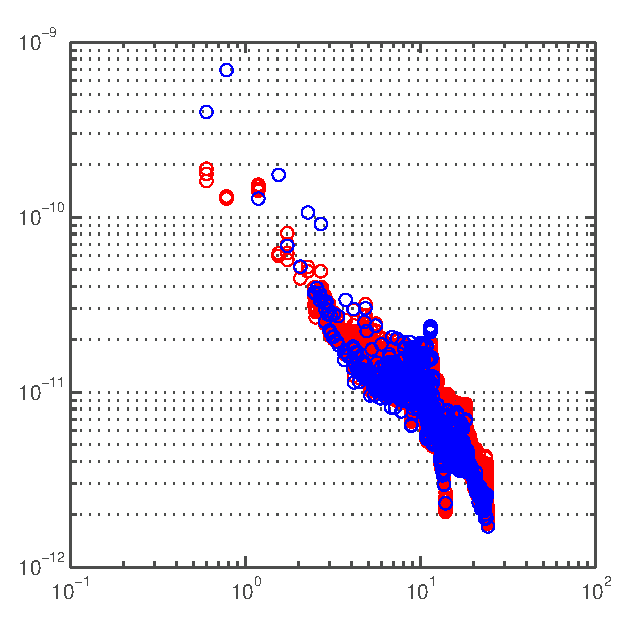
\includegraphics{/home/schuberm/Dropbox/git/plots.nogit/images/NMD_v_ALD.eps}}
\renewcommand{\figure}{Fig.}
\caption{Comparison between lifetimes from NMD and ALD in a $4\times4$ superlattice without interfacial mixing.}
\label{FIG:NMD_v_ALD}
\end{center}
\end{figure}
%%%
%Confirm the validity of ALD
Figure~\ref{FIG:NMD_v_ALD} shows no systematic bias between ALD and NMD for shorter lifetimes, with some systematic scatter at the longer lifetimes towards ALD. In general, ALD lifetimes are expected to be larger than NMD lifetimes because ALD neglects the contribution from $n$ order phonon processes\cite{PhysRevB.79.064301,esfarjani2011heat}, where $n$ is greater than 3.

\begin{table}
\begin{center}
\begin{tabular}{ccccc}
\hline\noalign{\smallskip}
&\multicolumn{3}{c}{$N\times N$ Superlattice} \\
\cline{2-5}\noalign{\smallskip}
\hspace{1cm} & $2\times2$ & $4\times4$ & $8\times8$ & $14\times14$  \\
\noalign{\smallskip}\hline\noalign{\smallskip}
$\tau_{eff}$   & 0.51 $\pm$ 0.51 & 0.49 $\pm$ 0.59 &  0.33 $\pm$ 0.34& 0.21 $\pm$ 0.22 \\
ALD   & 0 $\pm$ 0 & 0.11  $\pm$  0.14 &  0.09  $\pm$  0.07 & NA \\
\noalign{\smallskip}\hline
\end{tabular}
\end{center}
\renewcommand{\table}{Table.}
\caption{}
\label{TB:taud}
\end{table}

Uncertainty in the NMD and GK prediction of thermal conductivity was found by determining the effect of removing a single molecular dynamics seed upon the average estimate. From Table~\ref{TB:validate}, the predictions for superlattices without interfacial mixing lie within the uncertainty of one another. For superlattices with mixing, NMD predicts a lower in-plane thermal conductivity, differing systematically by about 20\% while the cross-plane predictions, however lie within the uncertainty. For the remainder of this work, the 80/20 system is used to discuss the effects of interfacial mixing upon phonon properties.
%%%
\begin{table}
\begin{center}
\begin{tabular}{lcc}
\hline\noalign{\smallskip}
&\multicolumn{2}{c}{Method} \\
\cline{2-3}\noalign{\smallskip}
$k$ & NMD  & GK  \\
\noalign{\smallskip}\hline\noalign{\smallskip}
Cross-Plane Perfect  & 0.26 $\pm$ 0.001& 0.26 $\pm$ 0.02\\
Cross-Plane 80/20    & 0.17  $\pm$ 0.001   &   0.18 $\pm$ 0.01 \\
Cross-Plane 60/40    & 0.18  $\pm$ 0.001   &   0.19 $\pm$ 0.01 \\
In-Plane Perfect   & 0.54 $\pm$ 0.005 & 0.53 $\pm$ 0.03  \\
In-Plane 80/20  & 0.25 $\pm$ 0.002 & 0.30 $\pm$ 0.01  \\
In-Plane 60/40   & 0.20 $\pm$ 0.002 & 0.26 $\pm$ 0.01  \\
\noalign{\smallskip}\hline
\end{tabular}
\end{center}
\renewcommand{\table}{Table.}
\caption{A comparison of the thermal conductivity predictions [$Wm^{-1}K^{-1}$] predictions for a $4\times4$ superlattice.}
\label{TB:validate}
\end{table}
%%%
%%%
\renewcommand{\textfraction}{0.0}
\begin{figure}%[H]
\begin{center}
\scalebox{1}{ \includegraphics{/home/schuberm/Dropbox/git/plots.nogit/images/lifvomega.eps}}
\renewcommand{\figure}{Fig.}
\caption{Lifetimes for perfect and mixed systems. From top to bottom $2\times2$, $4\times4$, $8\times8$ and $14\times14$ superlattices. The black line corresponds to the Ioffe-Regel criterion, $2\pi\omega^{-1}$. The brown line corresponds to a $A_2\omega^{-2}$ fit. The green line corresponds to a $A_4\omega^{-4}$ fit.}
\label{FIG:lifetime}
\end{center}
\end{figure}
%%%
Phonon lifetime as a function of frequency is shown in Figure ~\ref{FIG:lifetime}. As interspecies mixing is introduced, there is a downwards shift in phonon lifetimes, particularly for the higher frequency modes of short period superlattices, shifting some modes below the Ioffe-Regel criterion. As the modes for a given superlattice have a plane wave structure, enforced by the harmonic solution during the lattice dynamics calculation, reaching the Ioffe-Regel criterion is an indication of not spatial localization but rather temporal localization. Similar trends in the variation of lifetimes with frequency, dipping below the Ioffe-Regel criterion at intermediate frequencies and recovering at higher frequencies, as first observed in alloys \cite{jason2013vc}.

A Rayleigh scattering scaling ($\omega^{-4}$) is observed at larger frequencies for smaller period lengths ($2\times2$, $4\times4$), experienced by long wavelength phonons as a result of defect scattering \cite{PhysRev.140.A1812,klemens_scattering_1955-3,klemens_thermal_1957-2}. Rayleigh scattering is seen with photons in particular superlattices \cite{PhysRevLett.58.2486}. However, because the determination of $\tau\kv$ does not distinguish between phonon scattering mechanisms, the $\omega^{-4}$ scaling diverges at low frequencies and is replaced by $\omega^{-2}$ scaling. For the larger period length superlattices ($8\times8$, $14\times14$), the non-mixed systems have two distinct $\omega^{-4}$ scalings, particularly in the $14\times14$ superlattice but become smeared as interfacial mixing is introduced.

From Figure~\ref{FIG:MFP_cp}, there is a clear reduction in the contribution to cross-plane thermal conductivity from modes with a MFP greater than the period length as period length increases. This is consistent with the theoretical predictions from Mahan that a minimum occurs as the transport behaviour shifts from a wave-regime to particle-regime \cite{PhysRevLett.84.927,PhysRevB.56.10754}. This trend is not observed in the contribution curves for the in-plane conductivity (not shown), where the peak MFP remains unchanged as a function of period length. For short period superlattices, interfacial mixing shifts in the peak MFP towards shorter lengths and reduces its respective contribution. For mixed $2\times2$, $4\times4$ and $8\times8$, the peak MFP is shifted arbitrarily close to the period length, indicative of the transition of thermal transport from superlattice phonons to thermal transport from phonons, which may or may not map to the non-mixed dispersion, with MFP on the order of the period length. This trend further supports the fact that superlattice phonons become disrupted by interfacial mixing, thereby diminishing the wave effects of the secondary periodicity upon cross-plane thermal conductivity. At large enough period lengths, the effect of interspecies mixing has a negligible effect on phonon MFP, as the lifetimes become less affected with increasing period length (Figure~\ref{FIG:lifetime}).

%%%
\begin{figure}%[H]
\begin{center}
\scalebox{1}{ \includegraphics{/home/schuberm/Dropbox/git/plots.nogit/images/MFP_cp.eps}}
\renewcommand{\figure}{Fig.}
\caption{Phonon mean free path normalized by the period length contribution to the cross-plane thermal conductivity. From top to bottom $2\times2$, $4\times4$, $8\times8$ and $14\times14$ superlattices.}
\label{FIG:MFP_cp}
\end{center}
\end{figure}
%%%

A computational limitation of NMD is the challenge in resolving longer wavelength modes because of the limited resolution of the Brillouin zone enforced by the MD domain. This effect is observed in Figure~\ref{FIG:MFP_cp}, where the finite number of resolved wavevectors leads to what would appear as noise in the contribution distribution at longer MFPs. Although size-independent thermal conductivity was achieved, careful analysis of these longer wavelength modes would be beneficial. This has been observed in other mode by mode techniques, such as the real space force constant extraction method used by Esfarjani \cite{PhysRevB.84.085204}, where the limited resolution manifested in the stepwise behaviour of thermal accumulation function.

%%%
\begin{figure}%[H]
\begin{center}
\scalebox{1}{ \includegraphics{/home/schuberm/Dropbox/git/plots.nogit/images/KvL_24814.eps}}
\renewcommand{\figure}{Fig.}
\caption{In-plane and cross-plane thermal conductivity as a function of superlattice period length.}
\label{FIG:NMD_v_GK}
\end{center}
\end{figure}
%%%

A comparison between the Green-Kubo and NMD thermal conductivity predictions for both in-plane and cross-plane directions is shown in Figure~\ref{FIG:NMD_v_GK}. For short period superlattices, the in-plane and cross-plane predictions approach the alloy limit. As described by Mahan, the minimum thermal occurs at a point where the average MFP is slightly greater than the period length. Although the thermal conductivity predictions from NMD and GK for systems without interfacial mixing agree, mixing introduces discrepancies that cannot be explained by statistical uncertainty (Table~\ref{TB:validate}). The eigenvectors were assumed to remain valid even with the introduction of interfacial mixing (the same set of eigenvectors were used in the NMD procedure for mixed and non-mixed $N\times N$). The consequences of such an assumption is observed in Figure~\ref{fig:sed}, where while for the modes at low and high frequency, the peaks remain well-defined, some intermediate frequency modes become noticeably perturbed. Fitting a Lorentzian was deemed suitable for these systems since coefficient of determination value for the most effected modes was about 0.9 \cite{Cowpe20081066}. Making the same assumption becomes increasingly questionable as the alloy limit is approached. The modified superlattice dispersion allows one to capture the effects of the secondary periodicity upon group velocities and lifetimes. However, interfacial mixing disrupts this secondary periodicity and thus alters the dispersion. As such, although some modes continue to propagate unperturbed in the mixed systems, others effectively cease to be represented by the superlattice dispersion. This is observed in the power spectrum of select modes as seen in Figure~\ref{fig:sed}, where some peaks continue to be pronounced, indicative that these modes are hardly perturbed, while others diverge from the perfect case and begin to pick up frequencies associated with other modes that are captured in the NMD. In other words, the superlattice phonons which emerge from the secondary periodicity are effectively \textit{transformed} by the interfacial mixing.

\section{Superlattice phonons}

Past literature has cited superlattices as a structure where coherent effects upon thermal transport are possible; the trend in thermal conductivity as a function of period length being used to justify such a claim \cite{PhysRevB.67.195311} \cite{}. Here we have reproduced comparable trends simply by adopting the correct phonon dispersion for our analysis, implying an equivalency between a dispersion effect and a coherence effect. By using MD, we do no impose any restrictions upon phonon dynamics but let the system move through phase space naturally and thus should adequately capture all classical effects.

In part, the ambiguity attached to the term \textit {coherent effects} stems from its association with exotic configurations of material, like porous silicon \cite{doi:10.1021/nl102918q} \cite{} where the secondary periodicity emerges from the introduction of the repeated holes. Coherent effects, for that matter, are found in bulk systems since coherence requires the constructive or destructive interference of waves.

Finally, by relying upon the BTE, any coherent effect is abstracted into the particle-as-a-particle interpretation. Thus, we believe, coherent effects or equivalently, dispersion effects, are of consequence when one cannot use the bulk material phonon properties as particles to predict thermal transport in a non-bulk system.

\section{Summary}

To summarize, we show the reduction in the contribution to cross thermal conductivity from MFP greater than the superlattice period as the period length is increased. Differences between in-plane and cross-plane components of group velocity are responsible for the respective differences between thermal conductivity. Phonon lifetimes in superlattices can be significantly reduced by interspecies mixing, as the secondary periodicity is disrupted, thus reducing in-plane and cross-plane thermal conductivity. 

\newpage
%\bibliographystyle{apsrev}
\bibliography{superlattice.bib}

\end{document}

